
\chapter{Applications of Multivariate Analysis in Metabolomics}

\section{Introduction}

\begin{doublespace}
This chapter details several varied applications of multivariate analysis
within the field of metabolomics, from the simplest examples of constructing
multivariate calibration models of \hnmr{} NMR spectral data for determination
of caffeine concentration in coffee, to more complex examples of multiblock
statistical modeling of joint \hnmr{} NMR and electrospray MS data. A final
note on the relationship between PCA scores-space class separations and OPLS-DA
model reliability is also presented to conclude the chapter.
\end{doublespace}

\section{\hnmr{} NMR Fingerprinting of Brewed Coffees}

\begin{doublespace}
To provide an initial illustration of the capabilities of the MVAPACK software
suite \cite{worley:acscb2014}, four roasts of brewed coffee were purchased from
a local coffee shop. In this study, \hnmr{} NMR and UV/Vis absorbance spectra
were collected in order to construct a multivariate calibration of \hnmr{} NMR
spectral information against caffeine concentration.
\end{doublespace}

\subsection{Materials and Methods}

\subsubsection{Coffee Sample Preparation}

\begin{doublespace}
Four freshly brewed roasts of coffee (Light, Dark, Medium Regular and Medium
Decaffeinated) were purchased from a local coffee shop. From each roast,
sixteen 1.2 mL samples were drawn while the coffee was still hot and stored
at $-80^\circ$C for 24 hours. The samples were then lyophilized at
$-50^\circ$C and 0.1 mBar for 24 hours and subsequently redissolved in 1.0 mL
of 99.8\% D$_2$O (Isotec, St. Louis, MO) without pH adjustment. Following
redissolution, the samples were centrifuged at 12,000 RPM and $25^\circ$C
for 5 minutes and 800 $\mu$L of the supernatant was collected into NMR tubes.
The samples were stored in their NMR tubes at $4^\circ$C for 36 hours prior
to data collection.
\end{doublespace}

\subsubsection{Caffeine Extraction}

\begin{doublespace}
Measurement of the caffeine concentration in each coffee roast was performed
based on previously outlined procedures \cite{belay:food2008}. Triplicate
standards of caffeine were made by dissolving 2.9 mg of caffeine
(Sigma-Aldrich, St. Louis, MO) into 100.0 mL of 99.5\% CH$_2$Cl$_2$
(Sigma-Aldrich, St. Louis, MO) for a final concentration of 149 $\mu$M.
From each purchased coffee roast, 25 mL of brewed coffee were combined with
25 mL of CH$_2$Cl$_2$ in a separatory funnel in a two-step liquid-liquid
extraction. Extracted caffeine in CH$_2$Cl$_2$ was diluted 20-fold into 1.0
mL and subjected to UV/Vis absorption spectroscopy for caffeine quantitation.
\end{doublespace}

\begin{figure}[ht!]
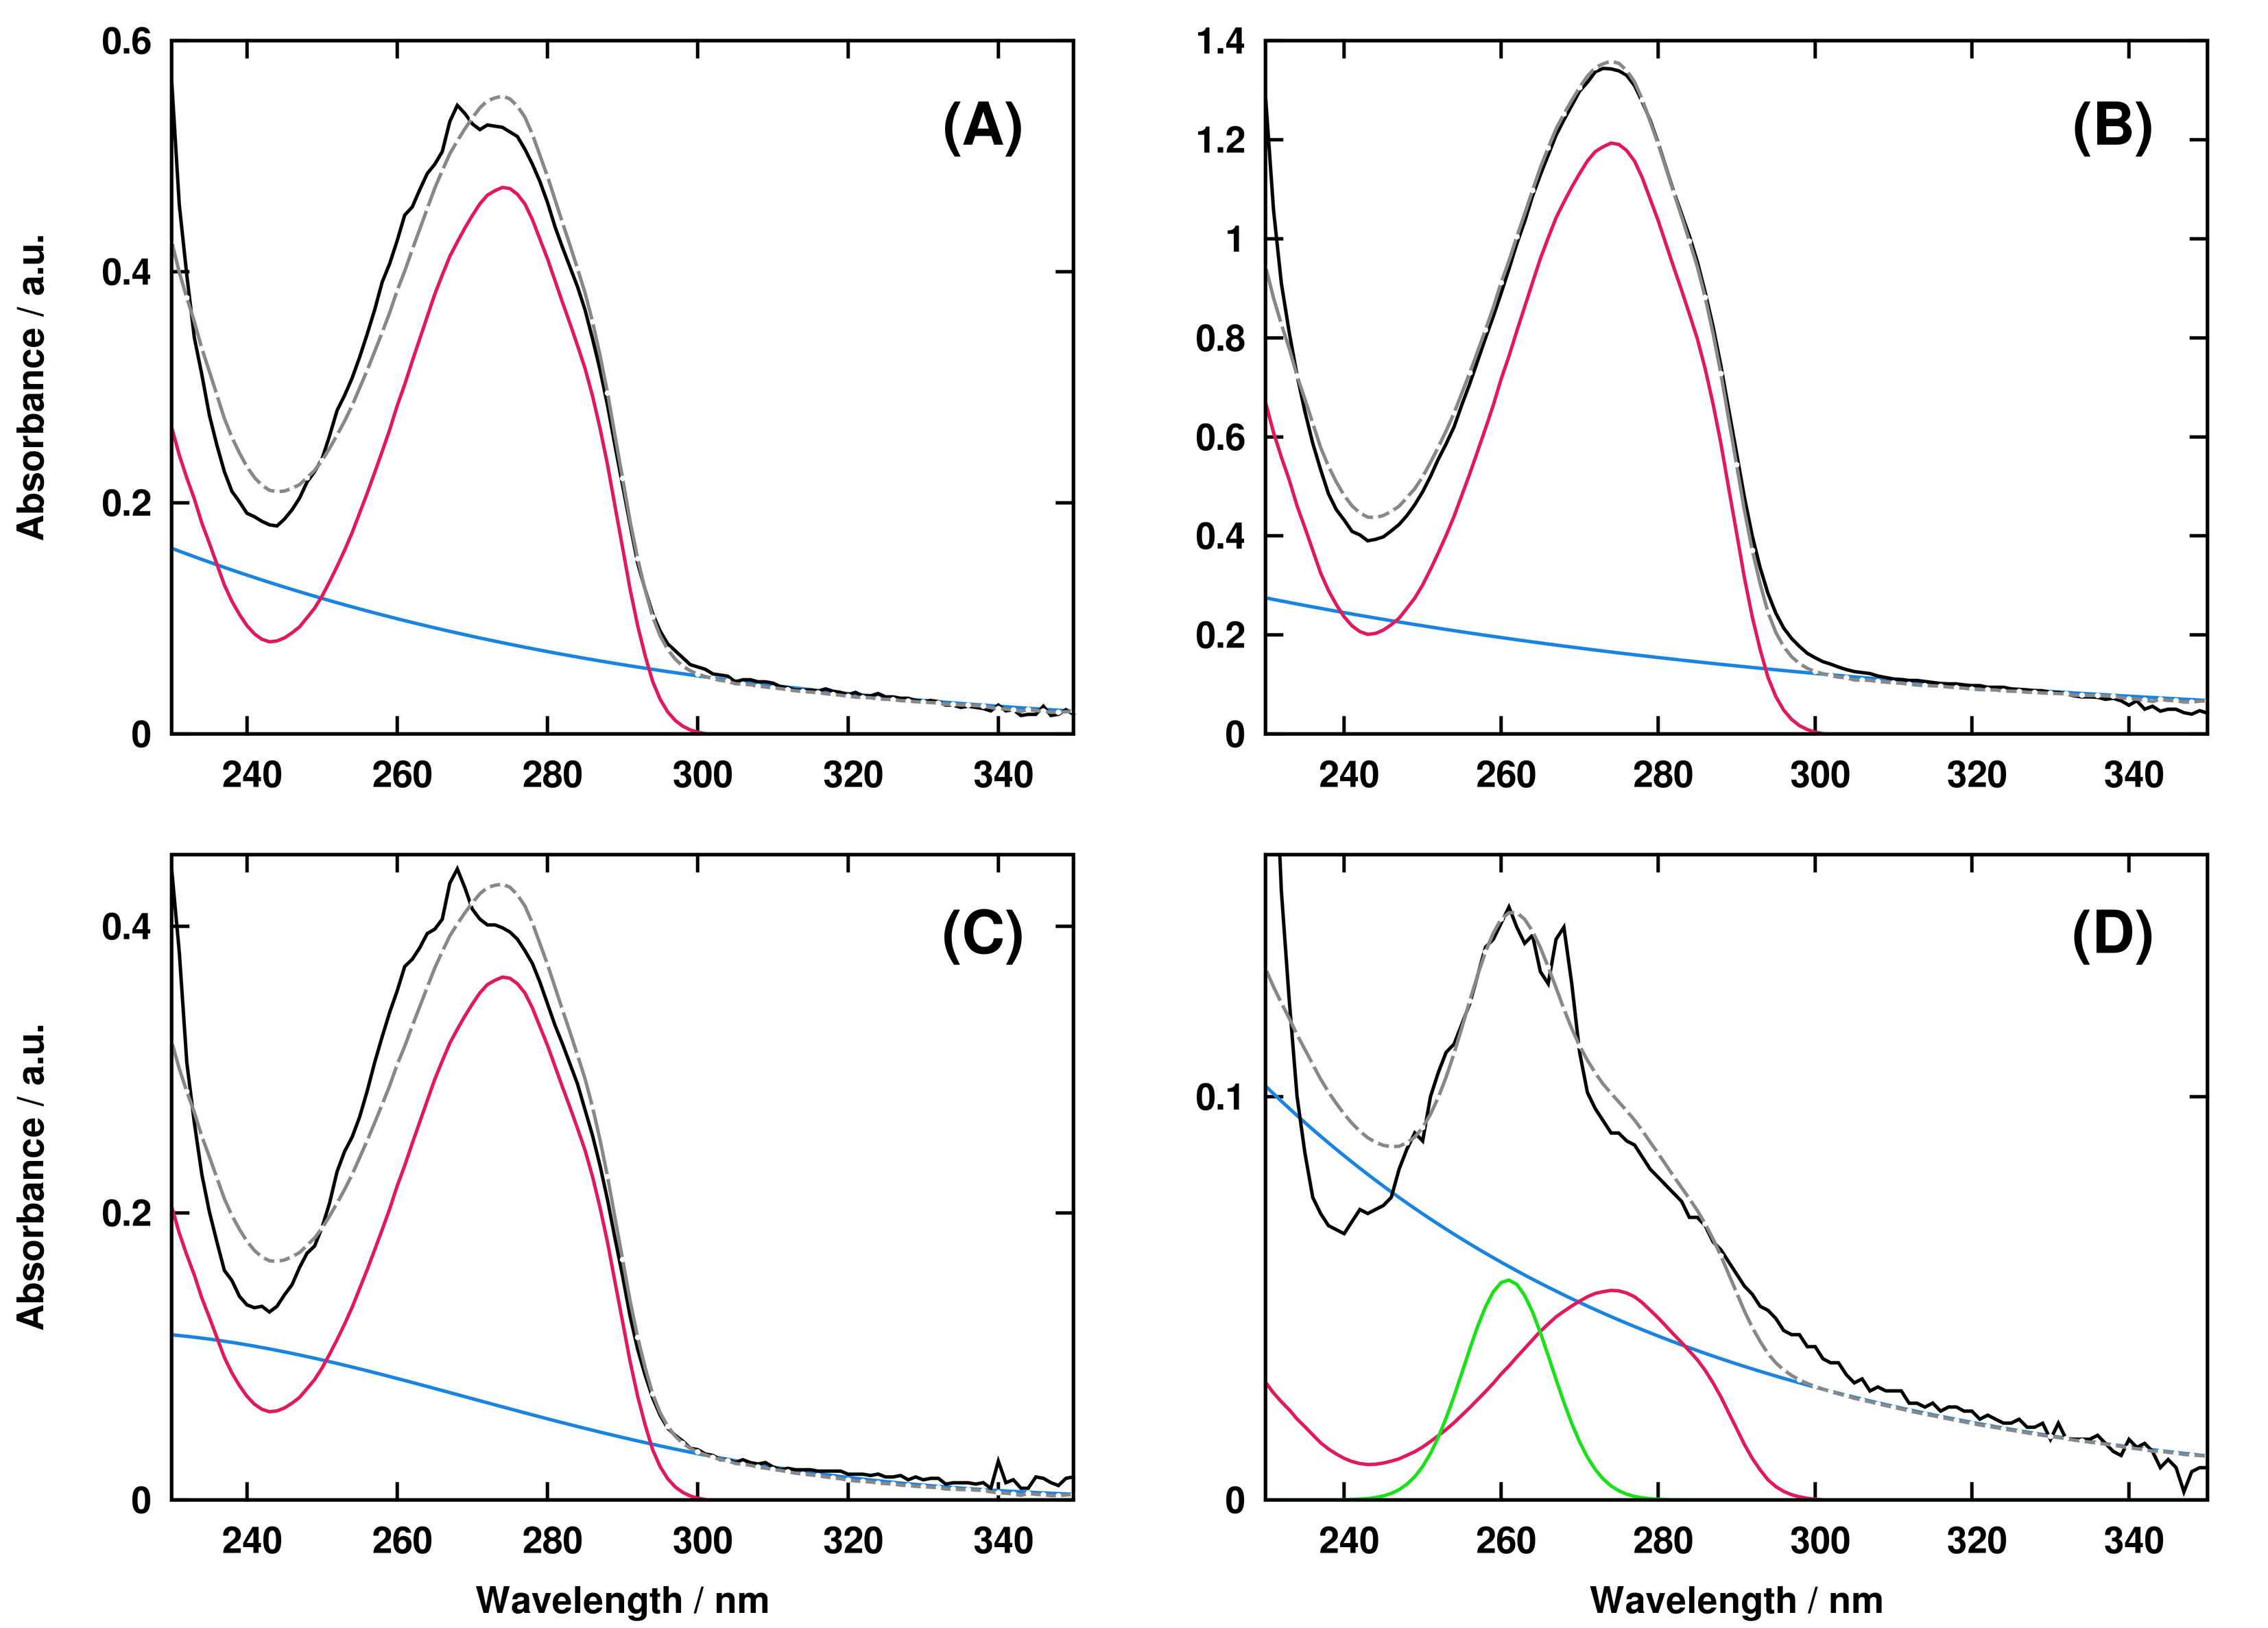
\includegraphics[width=6.5in]{figs/apps/01-uvfit.png}
\caption
      [UV/Vis Caffeine Quantitation Band-fitting Results.]{
  {\bf UV/Vis Caffeine Quantitation Band-fitting Results.}
  \\
  UV/Vis absorbance band-fitting results for caffeine concentration estimation
  of dark roast ({\bf A}), light roast ({\bf B}), regular medium roast
  ({\bf C}), and decaffeinated medium roast ({\bf D}). Black lines represent
  observed spectra, dashed grey lines represent fitted spctra, red lines
  represent fitted caffeine, and blue and green lines represent additional
  Gaussian bands required for fitting.
}
\end{figure}

\subsubsection{UV/Vis Spectroscopy}

\begin{doublespace}
Absorption spectra of caffeine standards and extracts were collected on a
Shimadzu UV-2501PC with a 1.0 nm slit width and 1.0 cm quartz cuvettes. Spectra
were collected between the wavelengths of 500 nm and 230 nm.
\end{doublespace}

\subsubsection{NMR Spectroscopy}

\begin{doublespace}
All NMR experiments were collected on a Bruker Avance DRX 500 MHz spectrometer
equipped with a 5 mm inverse triple-resonance (\hnmr{}, \cnmr{}, \nnmr{})
cryoprobe with a $z$-axis gradient. A Bruker BACS-120 sample changer and
ICON-NMR software were used to automate NMR data collection. A standard 1D
\hnmr{} NMR spectrum using a SOGGY pulse sequence
\cite{hwang:jmr1995,nguyen:jmr2007} and a $T_2$-filtered 1D \hnmr{} NMR
spectrum using a $z$-filtered Carr-Purcell-Meiboom-Gill (CPMG) sequence
\cite{rastrelli:jacs2009} with an identical SOGGY water suppression element
were acquired for each sample. All experiments were performed at $20^\circ$C
with 128 scans, 32 dummy scans, a carrier frequency offset of 2350.6 Hz, a
6009.0 Hz spectral width, and a 1.0 s inter-scan delay. For $T_2$ filtered
spectra, 20 repetitions of a CPMG-$z$ element having a delay ($\tau$) of 5.0
ms were performed per scan, for a total filter time ($2n\tau$) of 200.0 ms.
Free induction decays were collected with 32,768 total data points resulting
in a total acquisition time of 10 minutes per experiment.
\end{doublespace}

\subsubsection{Caffeine Quantitation}

\begin{doublespace}
A reference spectrum of caffeine in CH$_2$Cl$_2$ was generated from the three
standard UV/Vis absorption spectra by taking the mean of the spectra after
multiplicative scatter correction (MSC, \cite{fearn:cils2009}). To quantify
caffeine in the extracts, the absorption spectrum of each extract was fit by
nonlinear least squares \cite{marquardt:jsiam1963} to the sum of the scaled
caffeine reference spectrum and no more than two extra `background' Gaussian
bands (Figure 4.1). The ratio of the fit caffeine reference spectrum in each
extract to that of the known samples was used as an estimate of caffeine
concentration in the extracts. Concentrations of the medium regular, medium
decaffeinated, dark and light roasts were 1.526 mM, 0.217 mM, 1.979 mM and
4.993 mM, respectively.
\end{doublespace}

\subsubsection{Multivariate Analysis}

\begin{doublespace}
All NMR spectra were loaded, processed, treated and modeled inside the GNU
Octave 3.6 programming environment \cite{eaton2008} using functions available
in the MVAPACK software suite for chemometrics \cite{worley:acscb2014}.
Free induction decays were loaded in from Bruker DMX binary format and
corrected for group delay errors by a circular shift of their time-domain
data points. All decays were Fourier transformed, automatically phase-corrected
and referenced to match the chemical shifts of caffeine with known database
values. Spectral regions upfield of 0.44 ppm and downfield of 9.16 ppm were
removed from the dataset, as they contained no informative signals. As solvent
resonances were adequately suppressed by the excitation sculpting pulse
sequence, no spectral regions were removed around the water resonance.
Figure 4.2 illustrates the final result of spectral processing of the coffees
dataset using MVAPACK.
\end{doublespace}

\begin{figure}[ht!]
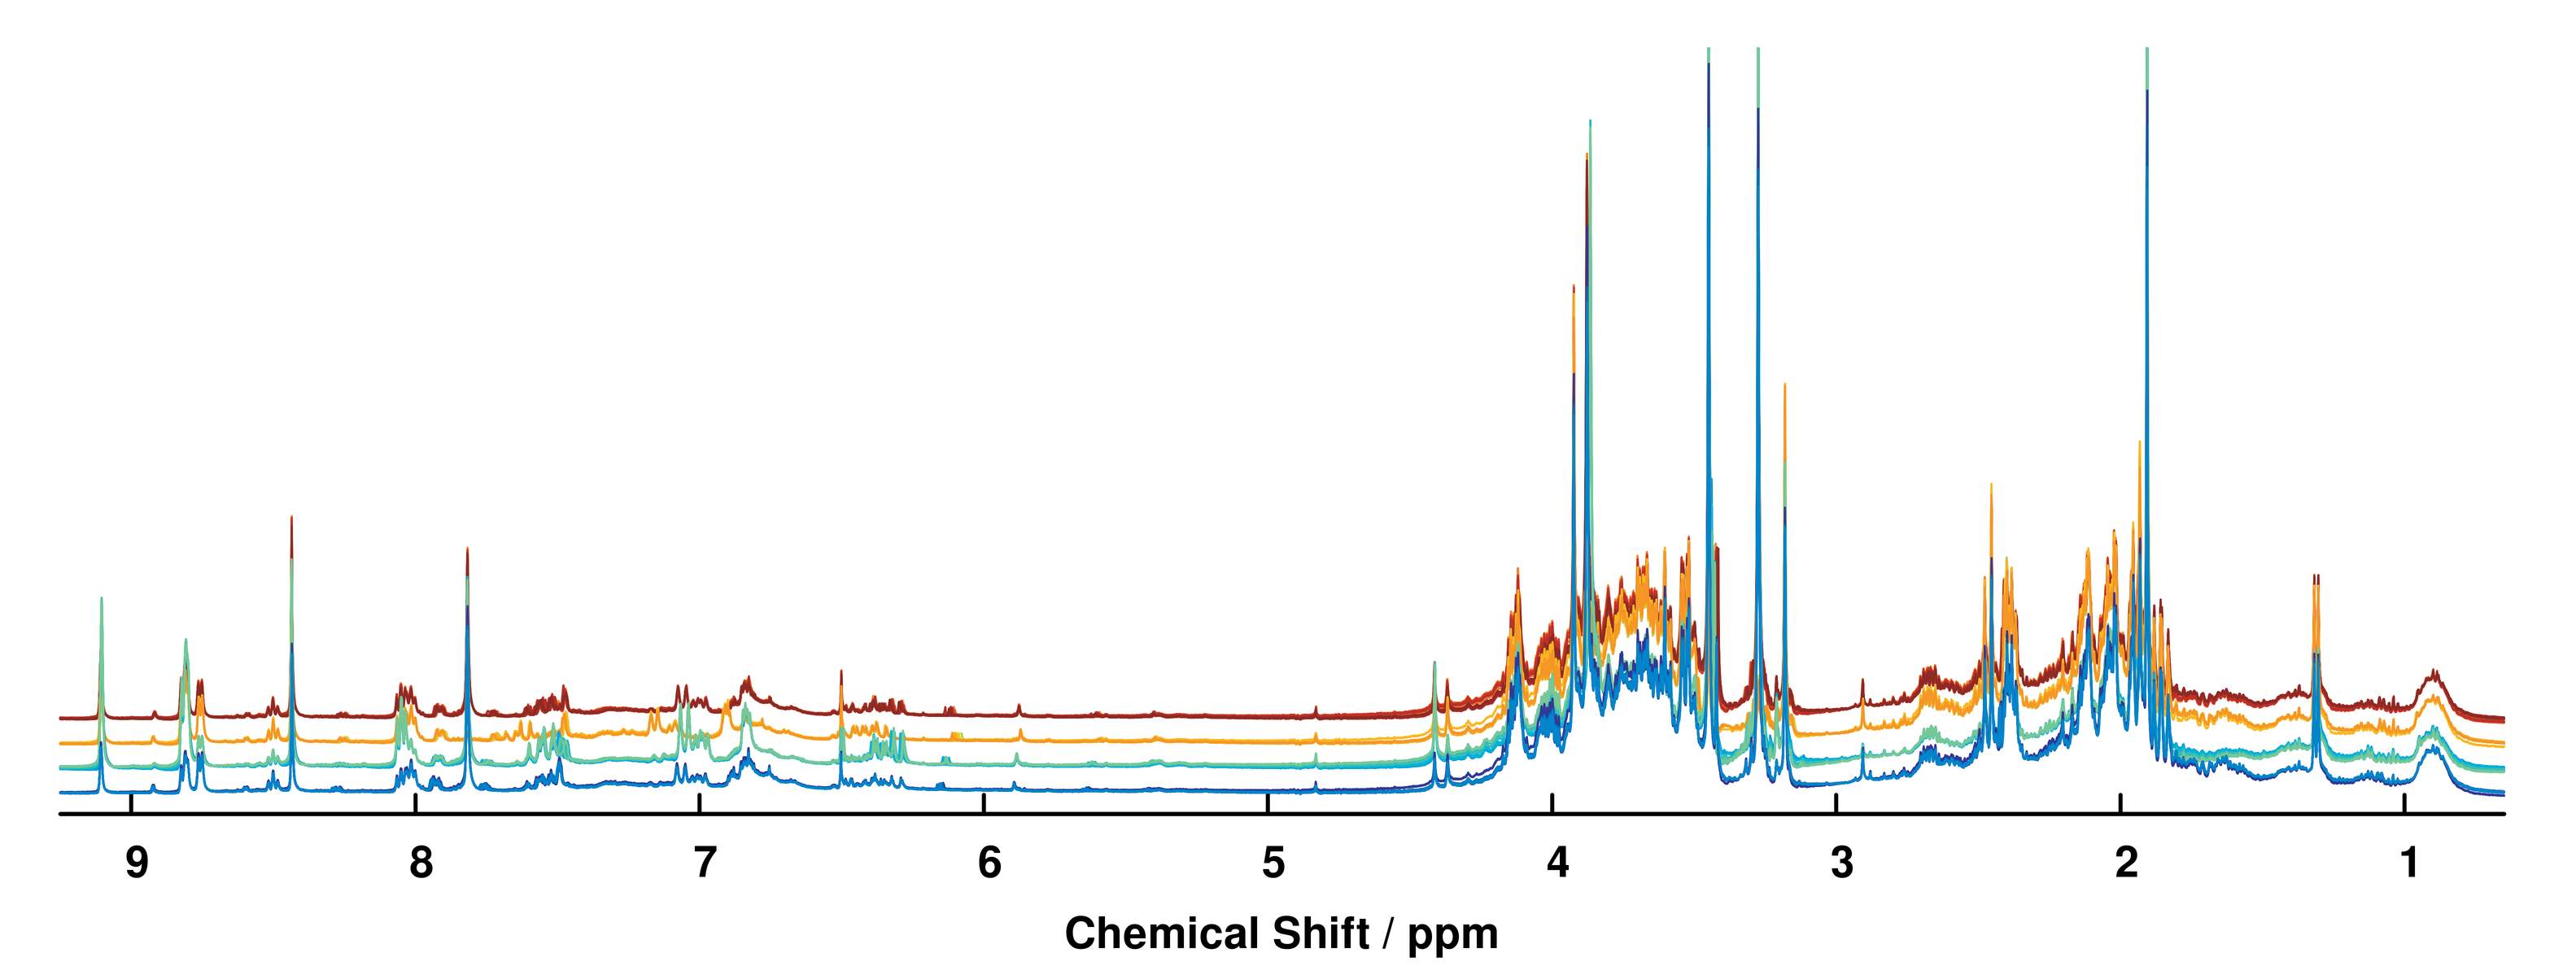
\includegraphics[width=6.5in]{figs/apps/02-spectra.png}
\caption
      [Processed \hnmr{} NMR Spectra of Coffee Roasts.]{
  {\bf Processed \hnmr{} NMR Spectra of Coffee Roasts.}
  \\
  Representative processed 1D \hnmr{} NMR spectra for all spectra of each
  coffee roast, acquired using the water-suppressed CPMG-$z$ pulse sequence
  and processed in MVAPACK. To reach this point, free induction decays were
  simply Fourier transformed and automatically phased. No manual phase
  corrections were applied after autophasing.
}
\end{figure}

\begin{doublespace}
For principal component analysis (PCA), the dataset was normalized by the
method of probabilistic quotients (PQ, \cite{dieterle:anchem2006}) and
subjected to adaptive intelligent binning \cite{demeyer:anchem2008}.
Low-variation `noise' bins were automatically removed from the dataset
\cite{zhang:opin2008}, resulting in a final data matrix having 64 observations
and 284 variables. The data matrix was scaled to unit variance
\cite{vandenberg:bmcg2006} prior to NIPALS PCA modeling \cite{jolliffe2002},
which produced six significant components having cumulative \rsqx{} and
\qsq{} statistics of 0.9689 and $0.8965 \pm 0.0105$, respectively
\cite{eshghi:cils2014}.
\\\\
Linear discriminant analysis (LDA) was performed on the first three dimensions
of resulting PCA scores to yield a two-component model that best
captured the between-class variation present in the three orthonormal PCA
score vectors. LDA modeling yielded a model having a cumulative \rsqx{}
statistic of 0.9950 and cumulative \rsqy{} and \qsq{} statistics of 1.0.
Scores from the PCA model of the coffees \hnmr{} NMR spectral data, and
their corresponding LDA projection, are shown in Figure 4.3.
\end{doublespace}

\begin{figure}[ht!]
\includegraphics[width=6.5in]{figs/apps/03-pca-lda.png}
\caption
      [Principal Component Scores of the Coffees Spectra.]{
  {\bf Principal Component Scores of the Coffees Spectra.}
  \\
  PCA ({\bf A}) and LDA ({\bf B}) scores of the four coffee roasts. Red,
  green, blue and violet points represent dark, light, decaffeinated medium,
  and regular medium roasts, respectively. Ellipsoids and ellipses enclose
  the 95\% confidence intervals estimated by the sample means and covariances
  of scores from each class. Axis labels in panels ({\bf A}) and ({\bf B})
  indicate scores in PCA and LDA bases, respectively, and not the same set
  of scores.
}
\end{figure}

\begin{doublespace}
For orthogonal projections to latent structures regression
(OPLS-R, \cite{trygg:jchemo2002}), the full-resolution dataset was aligned
using a per-class application of interval correlation-optimized shifting
(\emph{i}COshift, \cite{savorani:jmr2010}) and PQ normalization, resulting
in a final data matrix having 64 observations and 11,888 variables. The
Pareto-scaled data matrix was regressed by OPLS against a response vector
containing caffeine concentrations estimated by UV/Vis analysis of the four
coffee roasts, yielding a model with one predictive component and one
orthogonal component (\rsqxp{} = 0.5294, \rsqxo{} = 0.1288, \rsqy{} = 0.9822,
\qsq{} = $0.9502 \pm 0.0008$). CV-ANOVA significance testing returned a $p$
value equal to zero ($F$ = 2258.8) to within double-precision floating point
error, indicating a reliable model. The OPLS-R and LDA models were further
validated using response permutation tests having 1,000 iterations each. The
permutation tests of both models resulted in $p$ values less than 0.001 for
both \rsqy{} and \qsq{}, a further indication of high model reliability.
\end{doublespace}

\subsubsection{Validation against SIMCA-P+}

\begin{doublespace}
Correctness of the PCA and OPLS-R models generated by MVAPACK was verified by
exporting the final processed and treated data matrices from GNU Octave and
modeling them in SIMCA-P+ 13.0 (Umetrics AB, Umea, Sweden). The scores
extracted from SIMCA and MVAPACK were found to have coefficients of
determination (\rsq{}) of 0.999976 and 0.999989 for the PCA and OPLS models,
respectively. The `imperfect' non-unity values of \rsq{} reflect the fact that
SIMCA-P+ 13.0 only permits the export of scores with no more than four decimal
places.
\end{doublespace}

\subsection{Results and Discussion}

\begin{doublespace}
FIXME.
\end{doublespace}

\section{Fingerprinting of Joint \hnmr{} NMR and DI-ESI-MS Data}

\begin{doublespace}
FIXME \cite{marshall:metab2015}.
\end{doublespace}

\subsection{Materials and Methods}

\subsubsection{NMR Acquisition and Processing}

\begin{doublespace}
FIXME.
\end{doublespace}

\subsubsection{MS Acquisition and Processing}

\begin{doublespace}
FIXME.
\end{doublespace}

\subsubsection{Multivariate Statistical Analysis}

\begin{doublespace}
FIXME.
\end{doublespace}

\subsubsection{Cross-validation of Multivariate Models}

\begin{doublespace}
FIXME.
\end{doublespace}

\subsection{Results and Discussion}

\subsubsection{Data Treatment}

\begin{doublespace}
FIXME.
\end{doublespace}

\subsubsection{Classical Modeling}

\begin{doublespace}
FIXME.
\end{doublespace}

\subsubsection{Multiblock Modeling}

\begin{doublespace}
FIXME.
\end{doublespace}

\subsubsection{Metabolite Identification}

\begin{doublespace}
FIXME.
\end{doublespace}

\section{Monte Carlo Analysis of Scores-space Separations}

\begin{doublespace}
FIXME.
\end{doublespace}

\subsection{Materials and Methods}

\begin{doublespace}
FIXME.
\end{doublespace}

\subsection{Results and Discussion}

\begin{doublespace}
FIXME.
\end{doublespace}

\section{Conclusions}

\begin{doublespace}
FIXME.
\end{doublespace}

\bibliographystyle{abbrv}
\bibliography{bworley}

